%\documentclass[13pt]{amsart}
 \documentclass[%
    corpo=13pt,
    twoside,
%    stile=classica,
    oldstyle,
    autoretitolo,
    greek,
    evenboxes,
%    tipotesi,
]{toptesi}
\usepackage{pgfplots}       % it also load tikz package
\pgfplotsset{compat=1.17}   
\usetikzlibrary{arrows.meta, calc}
\usepackage{tikz}
\usetikzlibrary{positioning}
\usepackage{tcolorbox}
\usetikzlibrary{shapes.geometric, arrows, snakes, backgrounds, automata}
\tikzstyle{startstop} = [rectangle, rounded corners, minimum width=3cm, minimum height=1cm,text centered, draw=black, fill=red!30]
\tikzstyle{io} = [trapezium, trapezium left angle=70, trapezium right angle=110, minimum width=1cm, minimum height=1cm, text centered, draw=black, fill=blue!30]
\tikzstyle{process} = [rectangle, minimum width=1cm, minimum height=1cm, text centered, draw=black, fill=orange!30]
\tikzstyle{humprocess} = [rectangle, minimum width=1cm, minimum height=1cm, text centered, draw=black, fill=green!30]
\tikzstyle{decision} = [diamond, minimum width=1cm, minimum height=1cm, text centered, draw=black, fill=green!30]
\tikzstyle{arrow} = [thick,->,>=stealth]
%\tikzstyle{state} = [fill=blue!30]
\usepackage{tcolorbox}
\usepackage{caption}
\usepackage[colorlinks=true,
            citecolor={black}]{hyperref}
\usepackage{lipsum} % added for generating a dummy text, 
                    % not needed in real document
\usepackage{fancyvrb}
\begin{document}
\begin{comment}
\end{comment}
\tikzstyle{state}=[circle,draw=blue!50,fill=blue!20,thick]
\tikzstyle{transition}=[rectangle,draw=black!50,fill=black!20,thick]

			
%\filldraw [fill=black!30,draw=red] (semaphore.south -| enter critical.west) rectangle (waiting.north -| leave critical.east);
%REGEX NER
	\begin{figure}[ht] % placed here or on the top of page
		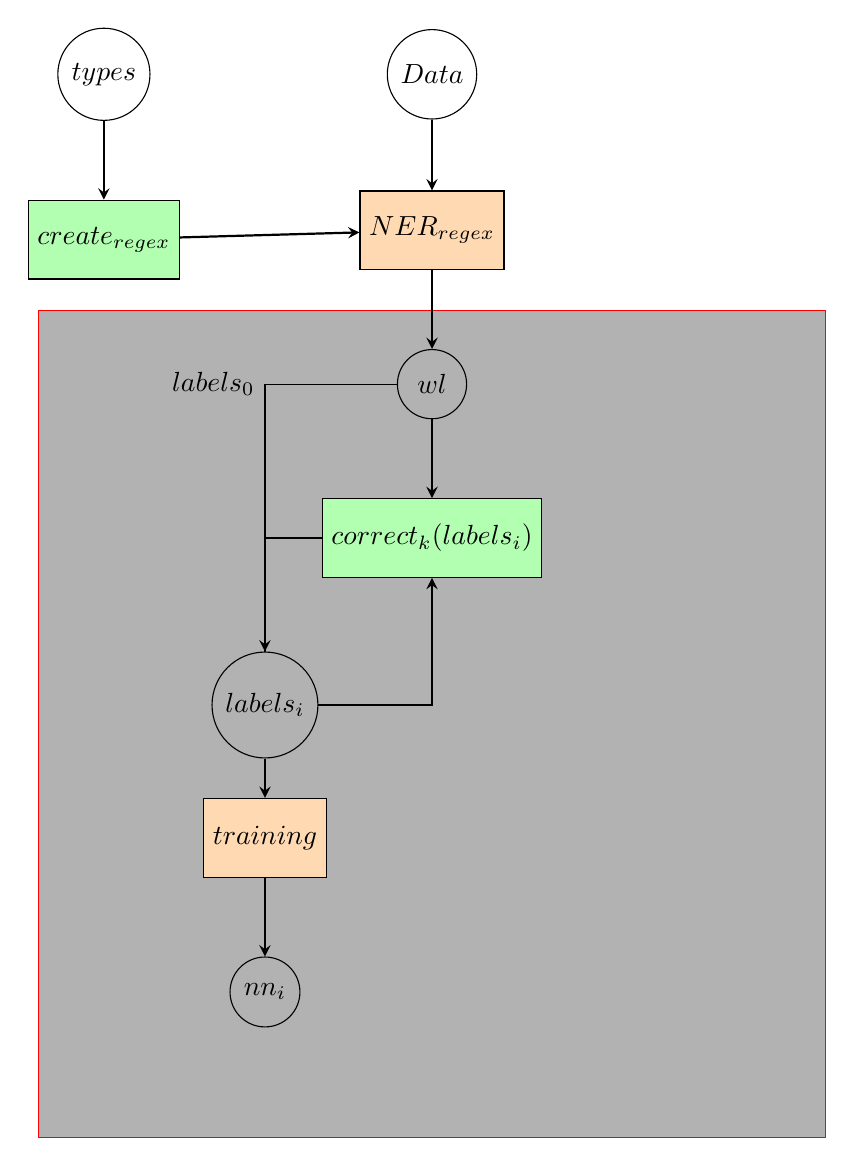
\begin{tikzpicture}[node distance=3cm]
		%\begin{tikzpicture}%[->,shorten >=1pt,auto,node distance=2.8cm,semithick]
			\node (data) [state] {\(Data\)};
			\node (regexner) [process, below=0.9cm of data] {\(NER\sb{regex}\)};
			\draw [arrow] (data) -- (regexner);
			\node (types) [state, left=3cm of data] {\(types\)};
			\node (humprod) [humprocess, below=1cm of types] {\(create\sb{regex}\)};			
			%\node (regex) [state, left=0.5cm of regexner] {\(R\sb{WL}\)};
			\draw [arrow] (types) -- (humprod);
			\draw [arrow] (humprod) -- (regexner);
			\node (wl) 		[state, below=1cm of regexner] {\(wl\)};
			\draw [arrow] (regexner) -- (wl);
			\node (humcorr) [humprocess, below=1cm of wl] {\(correct\sb{k}(labels\sb{i})\)};
			\draw [arrow] (wl) --  (humcorr) ;
			\node (l) 		[state, below left of=humcorr] {\(labels\sb{i}\)};
			%\draw [arrow] (humcorr) -- (l);
			    \draw  (wl) -- node[pos=1.5] {\(labels\sb{0}\)} ++(-2cm,0cm) -| (l) ;
			%\draw [arrow] (wl) --  ++(-2cm,0cm)-| (l); % node[pos=0.25] {2}  node[pos=0.75] {3};
			\draw [arrow] (humcorr) --  ++(-2cm,0cm)-| (l); % node[pos=0.25] {2}  node[pos=0.75] {3};
			\draw [arrow] (l) --  ++(+2cm,0cm)-| (humcorr); % node[pos=0.25] {2}  node[pos=0.75] {3};
			\node (train) 	[process, below=0.5cm of l] {\(training\)};
			\draw [arrow] (l) -- (train);
			\node (nn) 		[state, below=1cm of train] {\(nn\sb{i}\)};
			\draw [arrow] (train) -- (nn);
			%\node (module) [process, right of=nn] {\(NER\sb{NNi}\)};
			%\draw [arrow] (nn) -- (module);
			%\node (entities) [state, below of=module] {\(Entities\)};
			%\node (entitiescorr) [state, above of=module] {\(labels\sb{i}\)};
			%\draw [arrow] (module) -- (entities);
			%\draw [arrow] (entitiescorr) -- (humcorr);
			
\begin{pgfonlayer}{background}
\filldraw [fill=black!30,draw=red] (5,-3) rectangle (-5,-13.5);
%\filldraw [fill=black!30,draw=red] (nn.south -| nn.west) rectangle (humcorr.north -| entitiescorr.east);
\end{pgfonlayer}
		\end{tikzpicture}
%		\caption{Human In The Loop framework} % caption
		%\label{fig:diagram}             % for referencing of figure, key select as you wish
	\end{figure}
%\lipsum[2]  % dummy textù


\end{document}